% !TEX root = ./Cours.tex
\documentclass[../€Cours-complet/Cours-complet]{subfiles}

\titleorchapter{Nombres relatifs}{5}

\begin{document}

\maketitle

\section{Définition des nombres relatifs}

\begin{cours}
	\begin{itemize}
		\item Un nombre \textbf{positif} est un nombre supérieur à 0. On le note avec le signe +, ou sans signe.
		\item Un nombre \textbf{négatif} est un nombre inférieur à 0. On le note avec le signe −.
		\item Les nombres positifs et négatifs forment les nombres \textbf{relatifs}.
	\end{itemize}
\end{cours}

\begin{exemple}
	\begin{itemize}
		\item $3{,}2$ est un nombre positif. On peut aussi le noter $+3{,}2$.
		\item $-5{,}3$ est un nombre négatif.
		\item $0$ est le seul nombre à la fois positif et négatif.
		\item Tous ces nombres ($3{,}2$, $-5{,}3$, $0$, et d'autres) sont des nombres relatifs.
	\end{itemize}
\end{exemple}

\section{Repérage sur une droite}

\begin{definition}[Droite graduée]
	Une \textbf{droite graduée} est une droite sur laquelle on a placé :
	\begin{itemize}
		\item Un point qu'on appelle une \textbf{\color{red} origine}, qui porte le nombre $0$ ;
		\item Un \textbf{\color{Green} sens}, représenté par une flèche ;
		\item Une \textbf{\color{blue} unité de longueur}, qu'on utilise pour marquer de nouveaux points à intervalles réguliers depuis l'origine.
	\end{itemize}

	\begin{tikzpicture}[scale=2]
		\draw[-{Latex[length=3mm, width=2mm]}] (-2.3,0) -- (3.2,0);
		\foreach \p in {-2,-1,0,1,2,3} {
				\draw (\p,0) -- (\p,-0.1) node[below] {$\p$};
			}
		\draw[red,->] (0,0.5) node[above] {Origine} -- (0,0.2);
		\draw[blue,<->] (0,-0.5) -- node[below] {Unité de longueur} (1,-0.5);
		\draw[Green,->] (2.7,0.5) node[above] {Sens} -- ++(0.3,-0.3);
	\end{tikzpicture}
\end{definition}

\newpage

\begin{cours}
	Chaque point d'une droite graduée correspond à un nombre relatif. On l'appelle \textbf{l'abscisse} de ce point.
\end{cours}

\section{Comparaison de nombres relatifs}

\begin{cours}
	Lorsqu'on place deux nombres relatifs sur une droite graduée, le plus petit est celui à \textbf{gauche}.
\end{cours}

\begin{exemple}
	\begin{tikzpicture}
		\draw[-{Latex[length=3mm, width=2mm]}] (-3.5,0) -- (2.7,0);
		\foreach \x in {-3,...,2} {
				\draw (\x,0) -- (\x,-0.2);
				\node at (\x,-0.8) {\x};
			}
		\node[red] (A) at (-3,0) {X};
		\node[blue] (B) at (1,0) {X};
	\end{tikzpicture} \hspace{2em}
	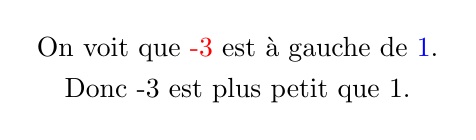
\begin{tikzpicture}
		\node (first_line) {On voit que {\color{red} -3} est à gauche de {\color{blue} 1}.};
		\node at ([yshift=-1.5em] first_line) {Donc -3 est plus petit que 1.};
	\end{tikzpicture}
\end{exemple}

\begin{methode}
	\begin{itemize}
		\item Si on a \myuline{deux nombres positifs} :

		      On sait déjà faire.
		\item Si on a \myuline{un nombre négatif et nombre positif} :

		      Le nombre négatif est toujours plus \textbf{petit} que le nombre positif.
		\item Si on a \myuline{deux nombres négatifs} :

		      \begin{tabular}{ll}
			      Le plus petit est & ∙ celui qui est le plus \textbf{loin} de zéro.                      \\
			                        & ∙ celui qui est le plus \textbf{grand} lorsqu'on enlève le signe -.
		      \end{tabular}
	\end{itemize}
\end{methode}

\begin{exemple}
	\begin{itemize}
		\item 1 est plus petit que 6. On note 1 < 6.
		\item 5{,}2 est plus grand que 5{,}1. On note 5{,}2 > 5{,}1.
		\item -3 est plus grand que -4, car 3 est plus \textit{petit} que 4. On note -3 > -4.
		\item -2{,}5 est plus petit que -2{,}3, car 2{,}5 est plus \textit{grand} que 2{,}3. On note

		      -2{,}5 > -2{,}3.
	\end{itemize}
\end{exemple}

\begin{greybox}[frametitle={Rappel : comparer des nombres à virgules}]
	Pour comparer des nombres à virgule :
	\begin{itemize}
		\item On compare les parties entières (avant la virgule). Si l'une est plus petite que l'autre, c'est fini.
		\item Sinon, on regarde les chiffres après la virgule un par un.

		      Le premier nombre à avoir un chiffre plus petit que l'autre, ou plus de chiffres, est le plus petit.
	\end{itemize}

	\begin{exemple}
		On compare 25{,}12 et 25{,}13 :

		\begin{itemize}
			\item 25 = 25, donc on passe au premier chiffre après la virgule.
			\item 1 = 1, donc on passe au deuxième chiffre après la virgule.
			\item 2 < 3, donc 25{,}12 < 25{,}13.
		\end{itemize}
	\end{exemple}
\end{greybox}

\section{Repérage dans un plan}

\begin{cours}
	Un \textbf{repère du plan} est formé de deux droite graduées de même origine. L'une est appelée \textbf{\color{red} axe des abscisses}, l'autre \textbf{\color{blue} axe des ordonnées}.

	Si les droites sont perpendiculaires, on dit que le repère est \textbf{orthogonal}.
\end{cours}

\begin{cours}
	Dans un repère du plan, chaque point est répéré par deux nombres relatifs : l'un sur l'axe des abscisses, l'autre sur l'axe des ordonnées. Ce sont ses \textbf{coordonnées}.

	On les note \textbf{(abscisse; ordonnée)}.
\end{cours}

\begin{exemple}
	\begin{tikzpicture}
		\draw[ultra thin,gray] (-4.5,-3.5) grid (5.5,4.5);

		\draw[thick,-{Latex[length=3mm, width=2mm]}] (-4.5,0) -- (5.5,0) node[above] {\color{red} axe des abscisses};
		\draw[thick,-{Latex[length=3mm, width=2mm]}] (0,-3.5) -- (0,4.5) node[right] {\color{blue} axe des ordonnées};

		\foreach \x in {-4,...,-1,1,2,3,4} {
				\draw[thick] (\x,0) -- (\x,-0.2);
				\node at (\x,-0.5) {\x};
			}

		\foreach \y in {-3,...,-1,1,2,3} {
				\draw[thick] (0,\y) -- (-0.2,\y);
				\node at (-0.5,\y) {\y};
			}

		\coordinate (Origine) at (0,0);
		\node at (-0.4,-0.4) {0};

		\foreach \name \x \y in {A/2/3,B/-2/2,C/-3/-2,D/2/-2,E/-2/0,F/0/1} {
				\coordinate (\name) at (\x,\y);
				\node at (\x,\y) {X};
				\coordinate (\name-abscisse) at (\x,0);
				\coordinate (\name-ordonnée) at (0,\y);
				\node at ([yshift=1em,xshift=-0.5em] \name) {\name};
			}

		\draw[red,dashed,ultra thick] (A) -- (A-abscisse);
		\draw[blue,dashed,ultra thick] (A) -- (A-ordonnée);
	\end{tikzpicture}

	\begin{itemize}
		\item Le point A a pour coordonnées ({\color{red} 2};{\color{blue} 3}).
		\item Le point B a pour coordonnées ({\color{red} -2};{\color{blue} 2}).
		\item Le point C a pour coordonnées ({\color{red} -3};{\color{blue} -2}).
		\item Le point D a pour coordonnées ({\color{red} 2};{\color{blue} -2}).
		\item Le point E a pour coordonnées ({\color{red} -2};{\color{blue} 0}).
		\item Le point F a pour coordonnées ({\color{red} 0};{\color{blue} 1}).
	\end{itemize}
\end{exemple}

\newpage

\section*{Bonus : hiérarchie des nombres}

On remarque que, avec les nombres relatifs, on a ajouté une nouvelle catégories de nombres !

Il existe ainsi plusieurs catégories de nombres, chacune ajoutant un nouveau \textit{type} de nombre :

\begin{itemize}
	\item Les nombres entiers, dits \textbf{naturels}. Ceux-ci contiennent $0, 1, 2, ⋯$.
	\item Les nombres entiers \textbf{relatifs}, qui contiennent $0, 1, 2, ⋯$ mais aussi $-1, -2, -3, ⋯$.

	      \warningbox{Dans le cours, le terme \textit{relatif} s'applique aussi aux nombres à virgules, mais pas ici.}
	\item Les nombres \textbf{décimaux} : ce sont les nombres à virgules, mais qui ont seulement un nombre fini de chiffres après la virgule. Par exemple, $2{,}1$,\ \ $5$ ou encore $-6{,}8$.
	\item Les nombres \textbf{rationnels} : ce sont les fractions.
	\item Les nombres \textbf{réels} : ce sont tous les nombres qui peuvent se placer sur une droite. Par exemple, pi (π) n'est pas un nombre rationnel (il ne peut pas s'écrire sous forme de fraction), mais c'est un nombre réel, égal à $3{,}141592⋯$
\end{itemize}

On peut schématiser cela par le diagramme suivant :

\begin{center}
	\begin{tikzpicture}[every node/.style={scale=0.85}]
		\draw (0,0) ellipse (2 and 1);
		\draw (0,0.5) ellipse (3.7 and 2);
		\draw (0,1) ellipse (5.4 and 3);
		\draw (0,1.5) ellipse (7.1 and 4);
		\draw (0,2) ellipse (8.8 and 5);

		\node at (0,0.7) {naturels};
		\node at (-0.9,0.1) {0};
		\node at (0,0.1) {1};
		\node at (0.9,0.1) {2};
		\node at (-0.6,-0.5) {50};
		\node at (0.6,-0.5) {3014};

		\node at (0,2.2) {relatifs};
		\node at (-1,1.7) {-1};
		\node at (1.2,1.7) {-76};
		\node at (-2.5,0.5) {-2689};

		\node at (0,3.7) {décimaux};
		\node at (-3,2.7) {0{,}8};
		\node at (2,2.8) {-89{,}127};

		\node at (0,5.2) {rationnels};
		\node at (-6,2) {$-\frac{6}{11}$};
		\node at (-3,4) {$\frac{1}{3}$};
		\node at (5,3.5) {$\frac{60}{859}$};

		\node at (0,6.7) {réels};
		\node at (-5,5) {$\sqrt{3}$};
		\node at (-2,6) {$\sqrt{2}$};
		\node at (3,6) {π};
		\node at (8,3) {$e$};
	\end{tikzpicture}
\end{center}

\end{document}